\chapter[CLS Update Meeting]{Update Meeting}
\section{Communities Living Sustainably}
A brief presentation and demonstration of the Simulation Model was presented to CLS on 26 March 2015.

\begin{figure}[htbp]
\centering
\frame{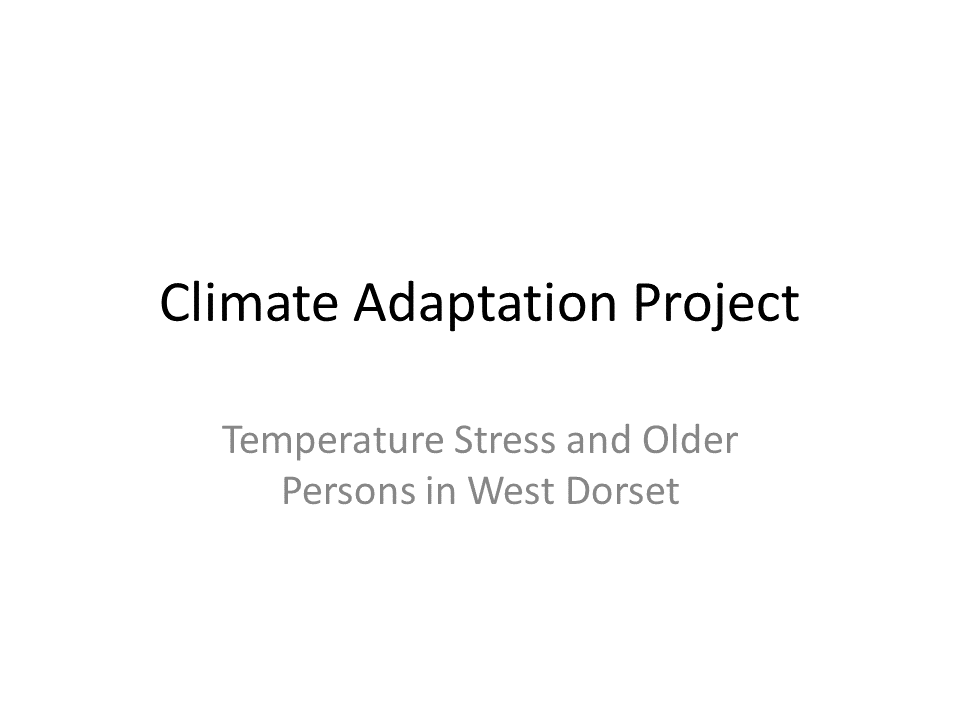
\includegraphics{img/clsSlide1.png}}
\caption[Update Talking Points Introduction]{We have begun to put together a visual model of what we believe will be the drivers of ill health in the older population resulting directly from climate change. We are limiting our exploration, at this time, to temperature stress.}
\end{figure}

\begin{figure}[htbp]
\centering
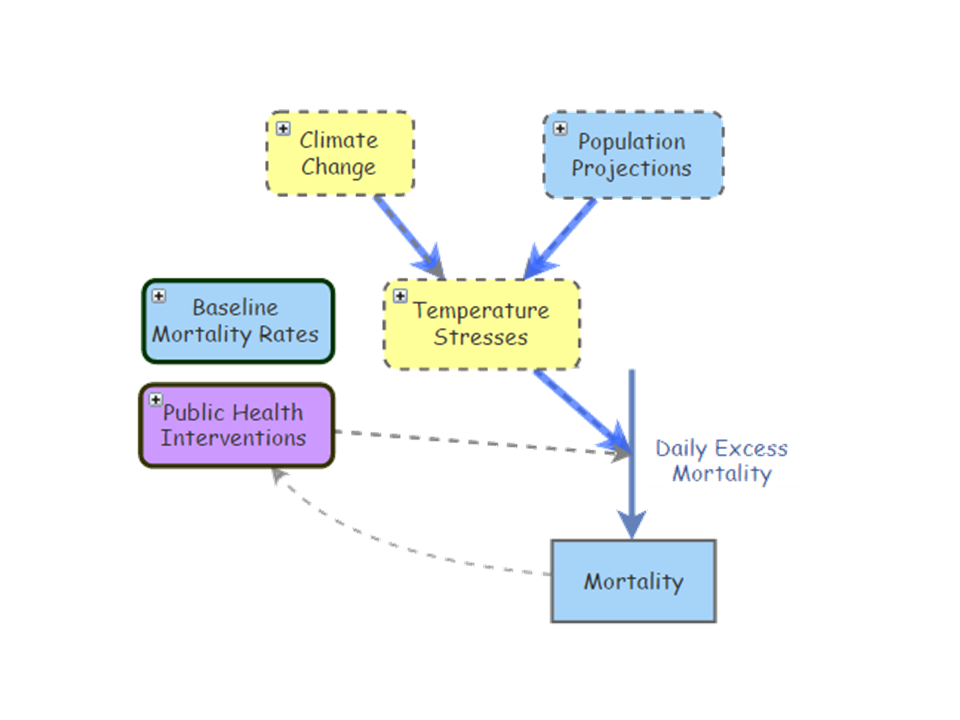
\includegraphics{img/clsSlide2.png}
\caption[Project Aim of Systems Model]{Our over-riding aim is to keep this model simple and hopefully `understandable'. Our causal pathway is that climate change will affect temperature stress and temperature stress impacts on daily mortality. We will also attempt to account for changing population demographics and the underlying base mortality rates of the West Dorset population.}
\end{figure}

\begin{figure}[htbp]
\centering
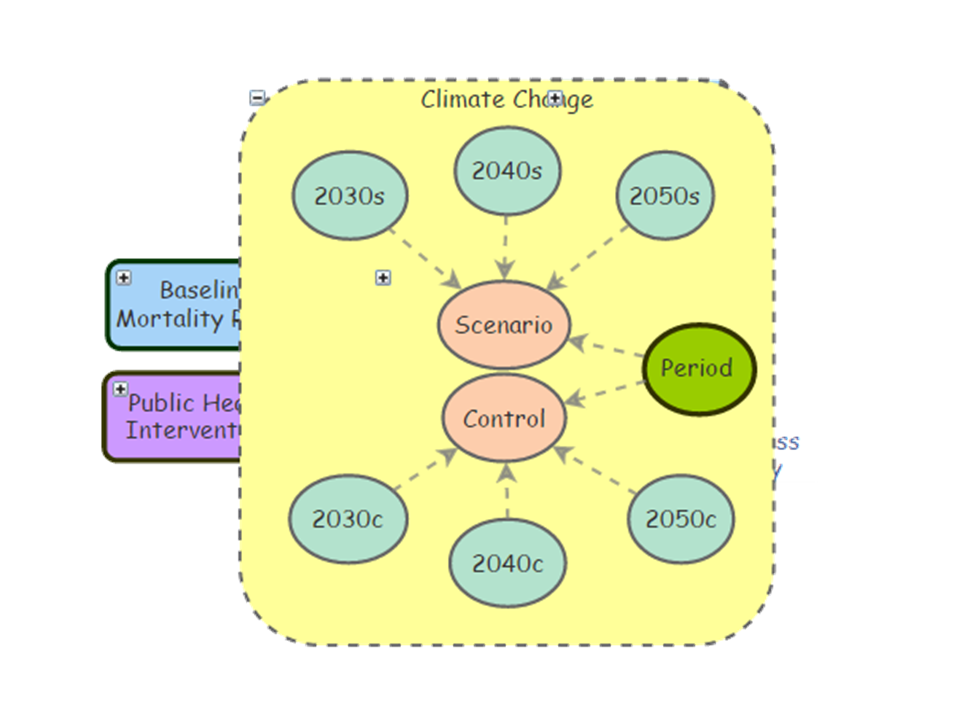
\includegraphics{img/clsSlide3.png}
\caption[Provision of Information `as needed']{Users can expand the climate change `folder' to inspect some of the model detail. We have set up the model to produce climate scenarios for three futures periods: 2030s, 2040s and 2050s. Each climate change scenario has a corresponding `control' simulation that produces `weather' for a typical contemporary period.}
\end{figure}

\begin{figure}[htbp]
\centering
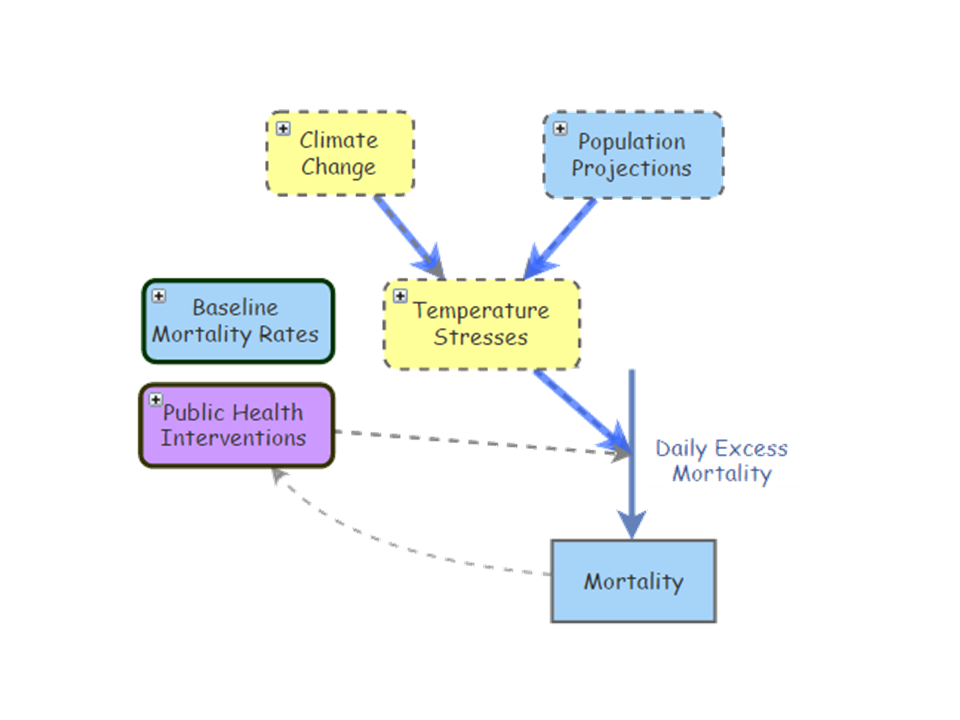
\includegraphics{img/clsSlide4.png}
\caption[Use of Folders in Model]{Folders are a component of the Insight Maker modelling system that allows one to control the level of detail visible immediately to the user. They access that detail by `clicking' on the `+' and can then hide the detail by clicking on the `-'.}
\end{figure}

\begin{figure}[htbp]
\centering
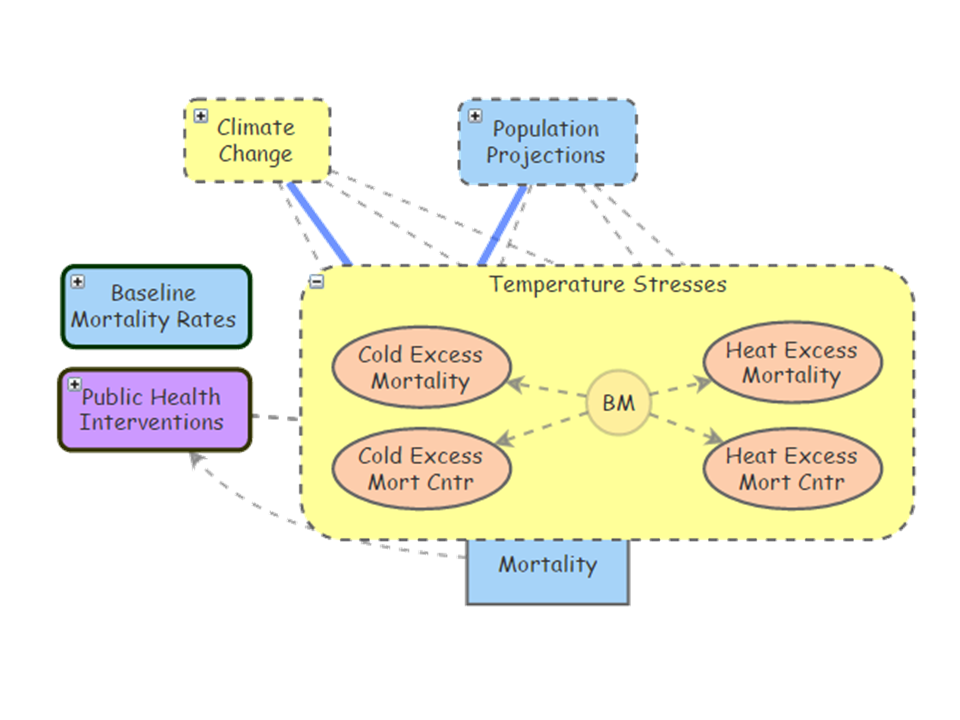
\includegraphics{img/clsSlide5.png}
\caption[Temperature Stress Explained]{Expanding the temperature stress folder reveals the process of calculating `excess mortality' from temperature stress, as informed by the underlying base mortality rates. This excess mortality is calculated as a relationship with temperature above (heat stress) and below (cold stress) a modelled regional threshold.}
\end{figure}

\begin{figure}[htbp]
\centering
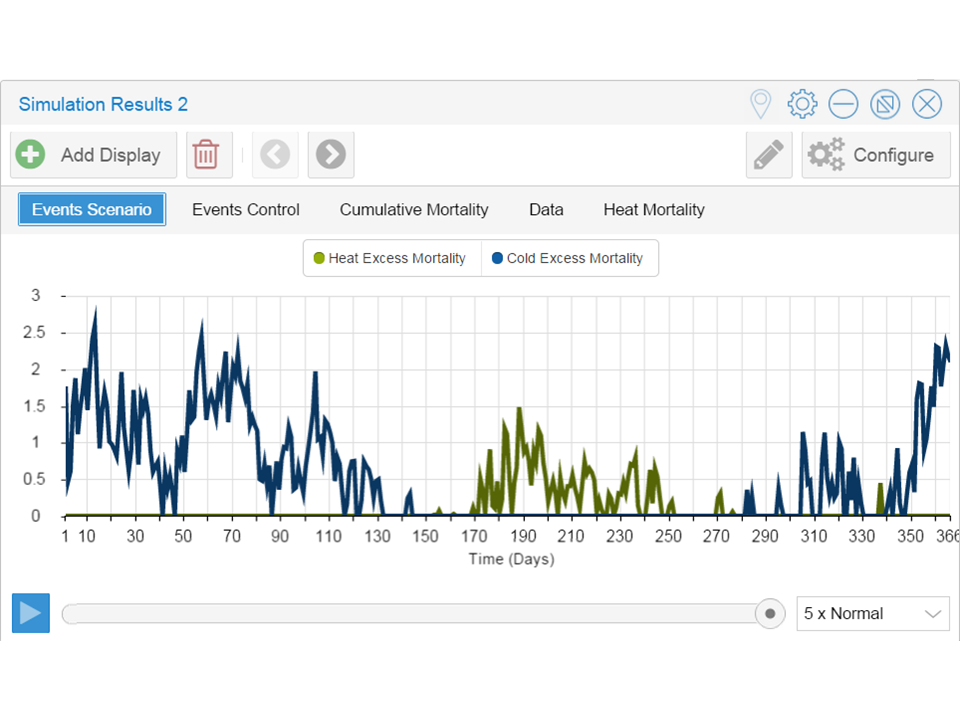
\includegraphics{img/clsSlide6.png}
\caption[Model Output Explained]{We have explored a number of ways in which to represent the dynamic simulation of future excess mortality. This graph illustrates the excess daily mortality over a `typical' year in sometime during the 20402. Cold stress mortality (blue line) flows into heat stress mortality (green line) and then back into colder periods, where day 1 is a hypothetical 1st of January and day 365 of the simulation is a hypothetical New Year's eve. The important insight is how much more cold stress mortality compared to heat stress -- even in the predicted warmer future.}
\end{figure}

\begin{figure}[htbp]
\centering
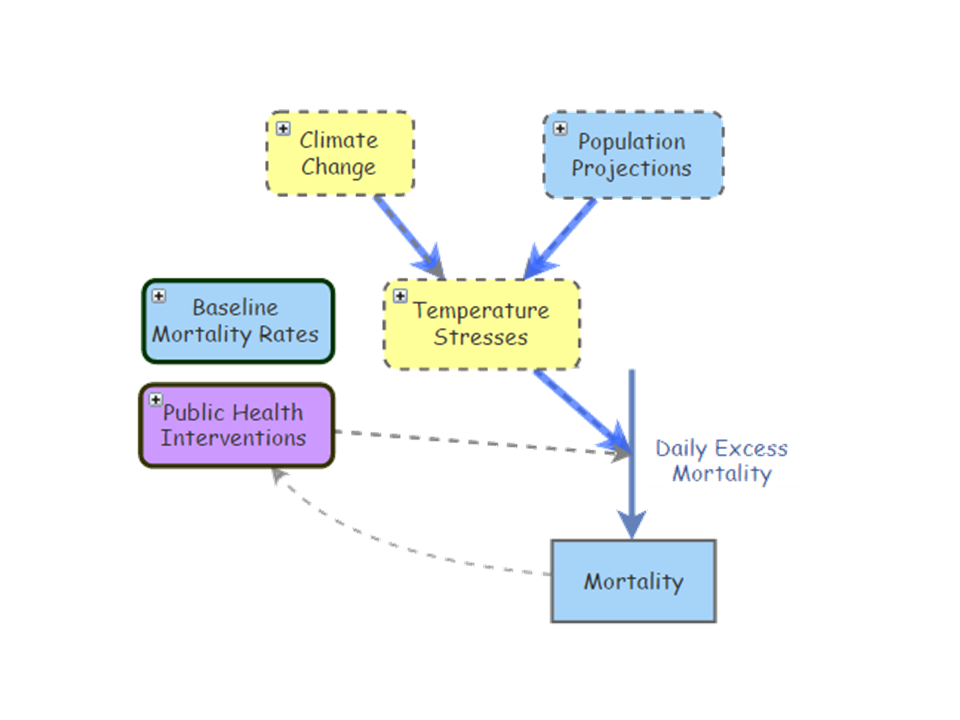
\includegraphics{img/clsSlide7.png}
\caption[Causal Pathway as a Communication Tool]{The causal pathway is clearly communicated when viewing the entire model, and the detail is available at the click of a mouse button. Baseline mortality is not in the causal pathway, but represents variables the model user can select.}
\end{figure}

\begin{figure}[htbp]
\centering
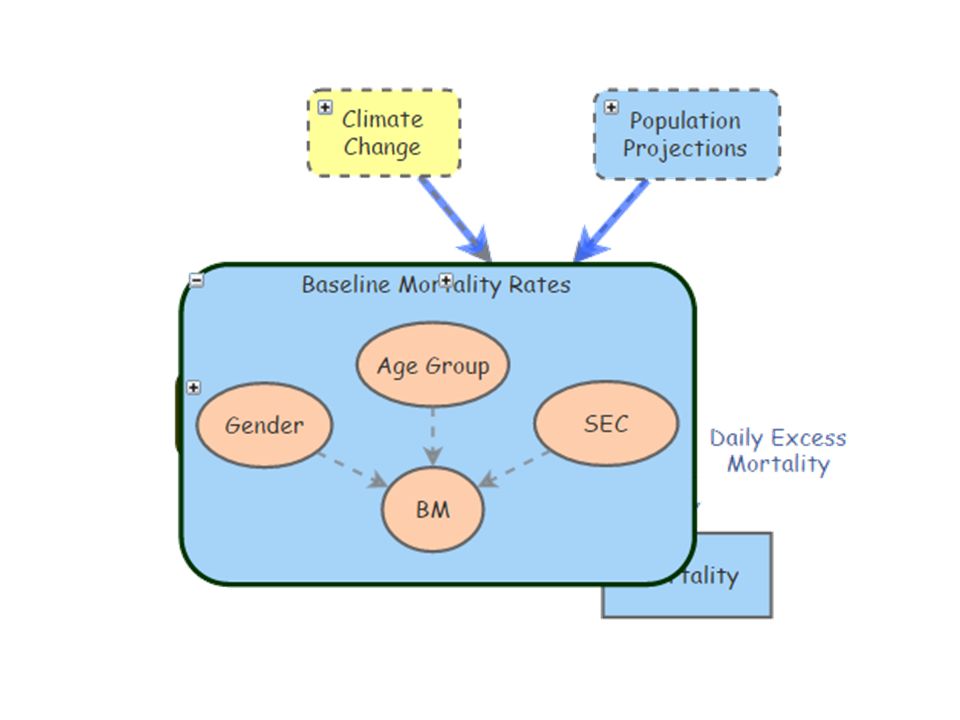
\includegraphics{img/clsSlide8.png}
\caption[ONS Base Mortality Explained]{ONS calculated baseline mortality varies significantly across gender, age, and seocio-economic status (SES).}
\end{figure}

\begin{figure}[htbp]
\centering
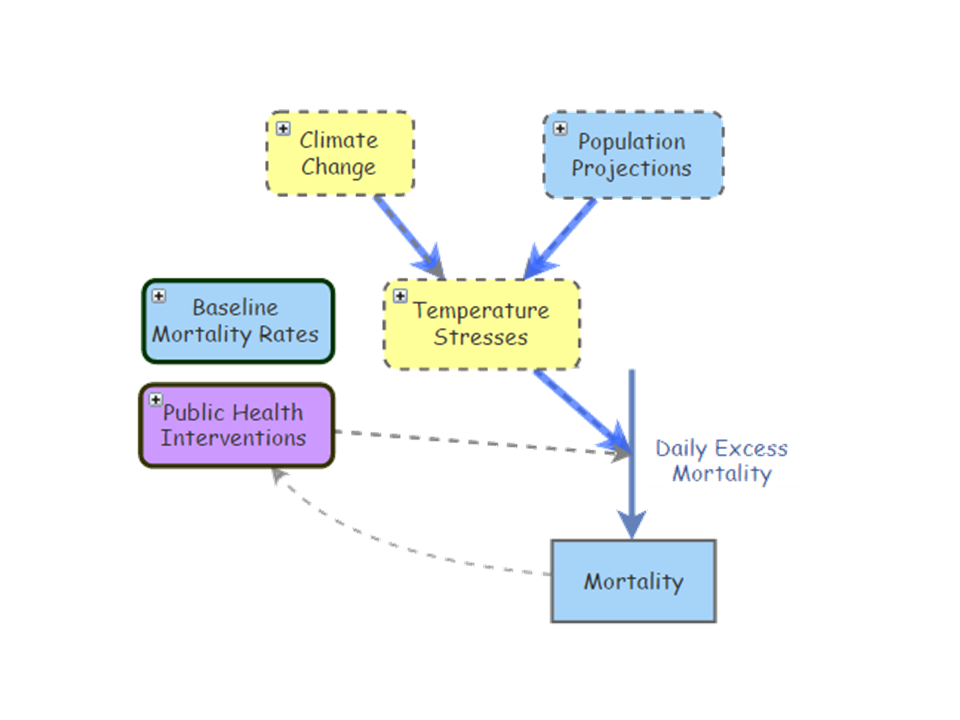
\includegraphics{img/clsSlide9.png}
\caption[Population Driver in System Model]{Population is also not in the causal pathway. Nonetheless, the underlying forecast changes to the demographic structure of the West Dorset population will impact the calculation of baseline mortality rates because this is an area that will experience fairly rapid growth in the 70+ age group population.}
\end{figure}

\begin{figure}[htbp]
\centering
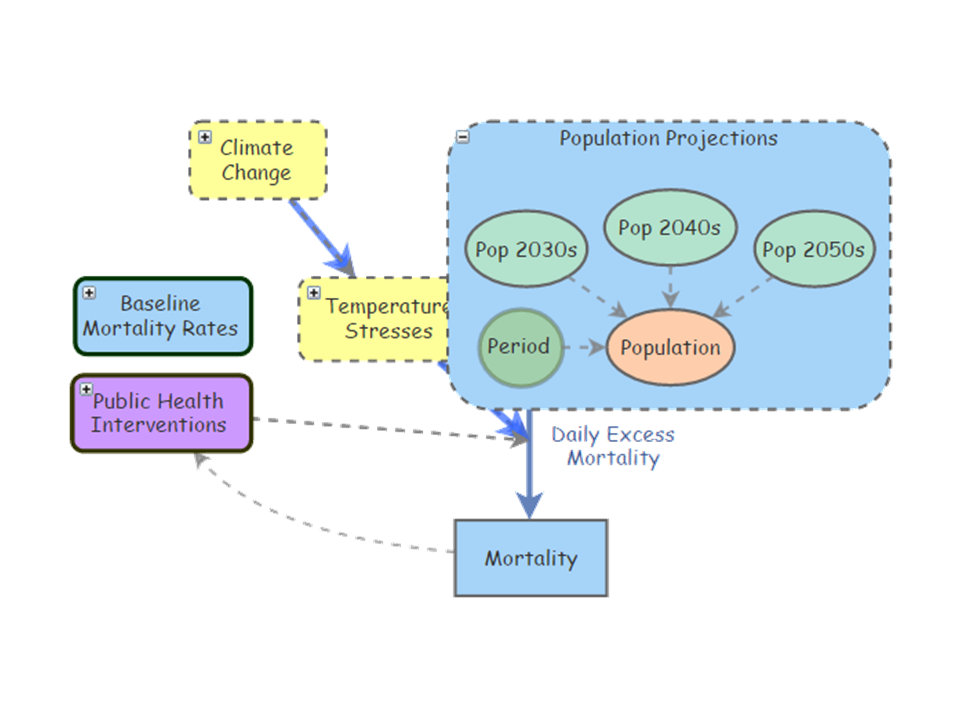
\includegraphics{img/clsSlide10.png}
\caption[Population Project Data Explained]{Examining the population project information in more detail shows that the model user selects the projects appropriate to the time period of the climate scenario already selected.}
\end{figure}

\begin{figure}[htbp]
\centering
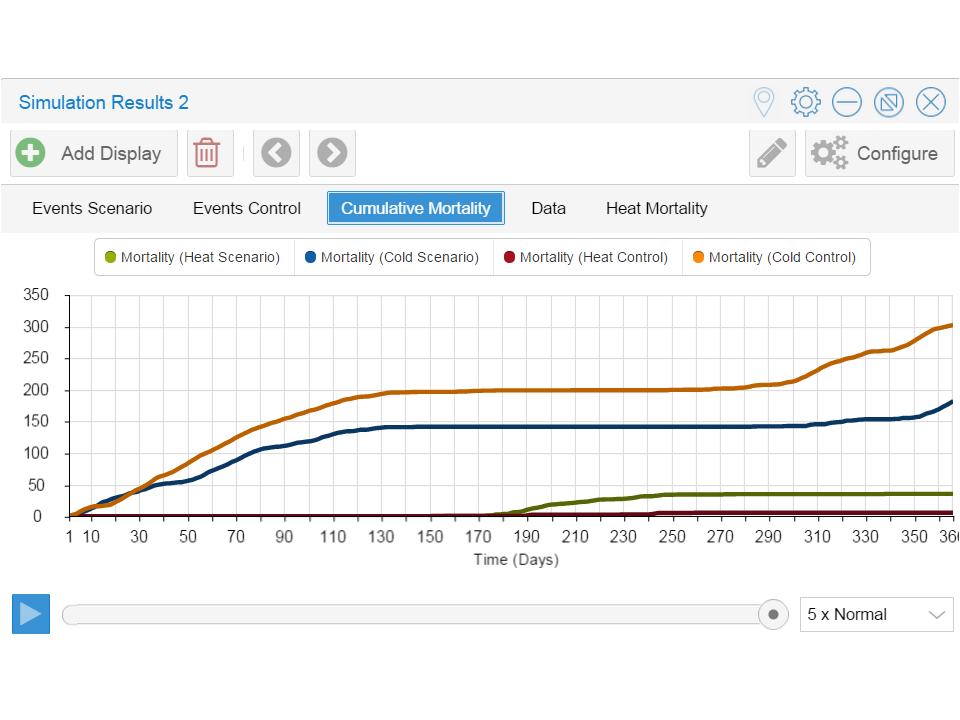
\includegraphics{img/clsSlide11.png}
\caption[Cumulative Mortality -- No Intervention]{The systems model provides a variety of graphical output that can be watched as the model runs. The output from this simulation is of all older people (70+) with no public health interventions.}
\end{figure}

\begin{figure}[htbp]
\centering
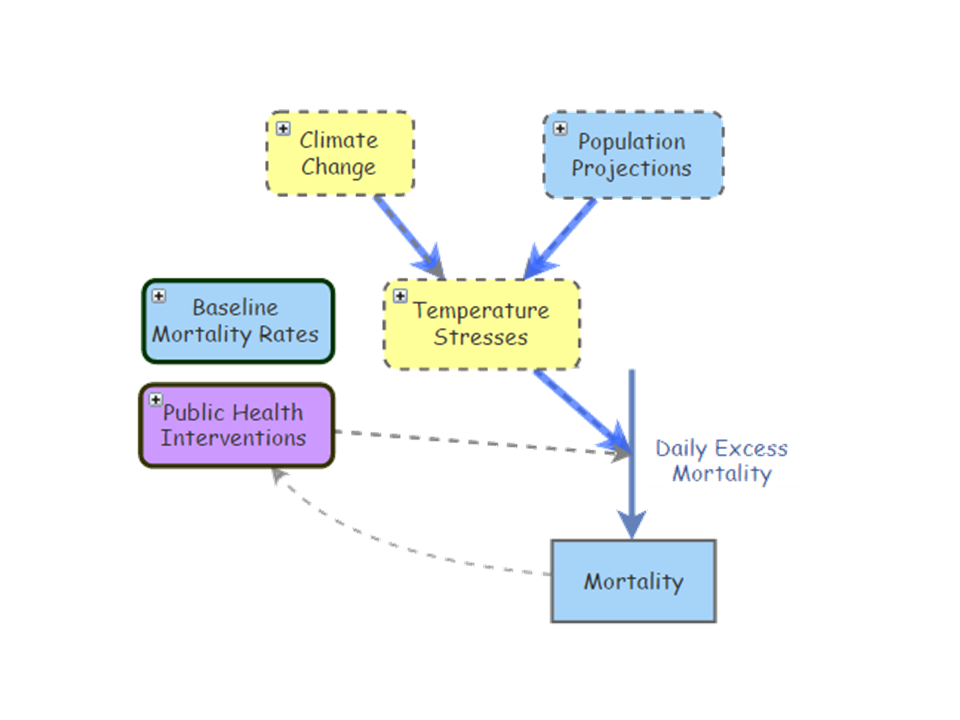
\includegraphics{img/clsSlide12.png}
\caption[Public Health Interventions]{There is scope, however, for introducing public health interventions into the simulation.}
\end{figure}

\begin{figure}[htbp]
\centering
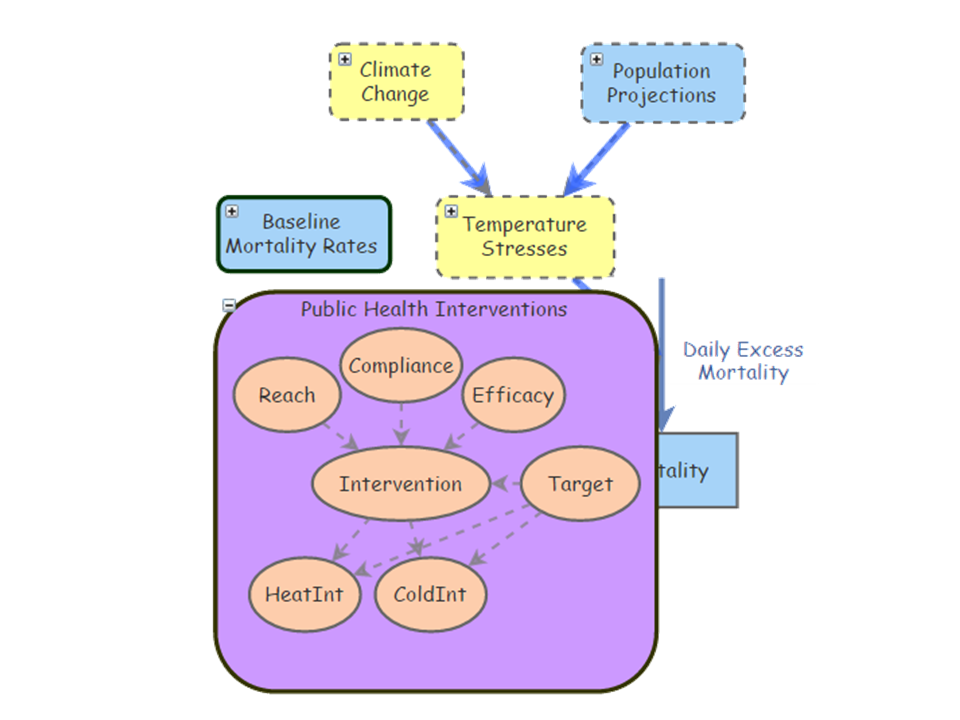
\includegraphics{img/clsSlide13.png}
\caption[Public Health Interventions Explained]{Public health interventions can be implemented by setting three elemental variables: reach, compliance and efficacy. The Target variable indicates whether the intervention is on cold or heat stress and the HeatInt and ColdInt are parameters used in the calculation they are not variable the user can set. }
\end{figure}

\begin{figure}[htbp]
\centering
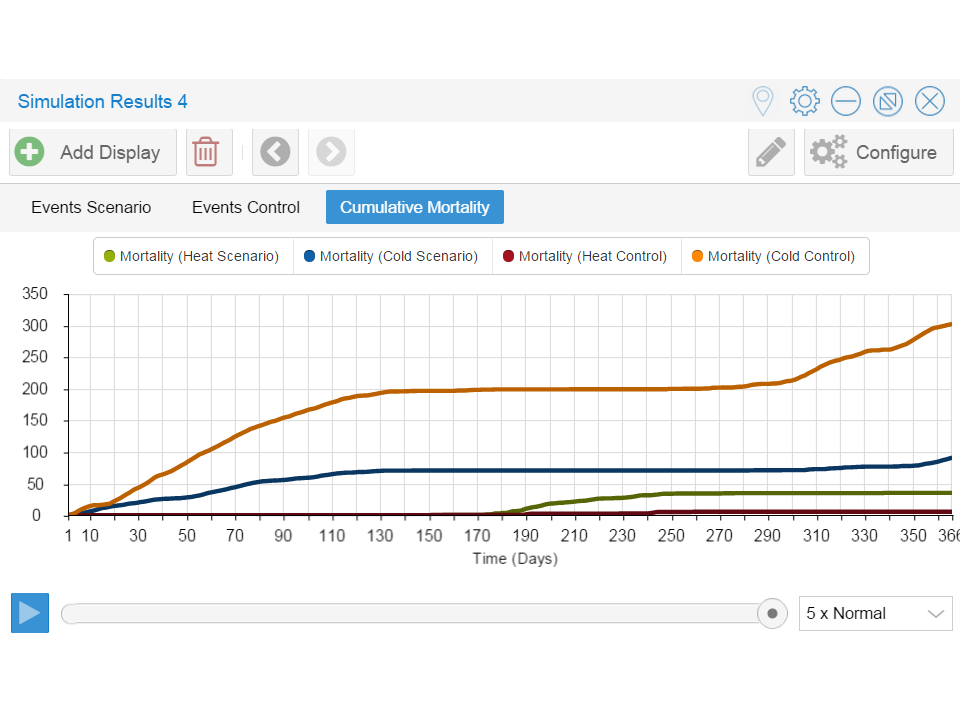
\includegraphics{img/clsSlide14.png}
\caption[Cumulative Mortality -- Cold Intervention]{A simulation with a cold intervention illustrates the reduced mortality compared with the previous `no intervention' simulation output.}
\end{figure}

\begin{figure}[htbp]
\centering
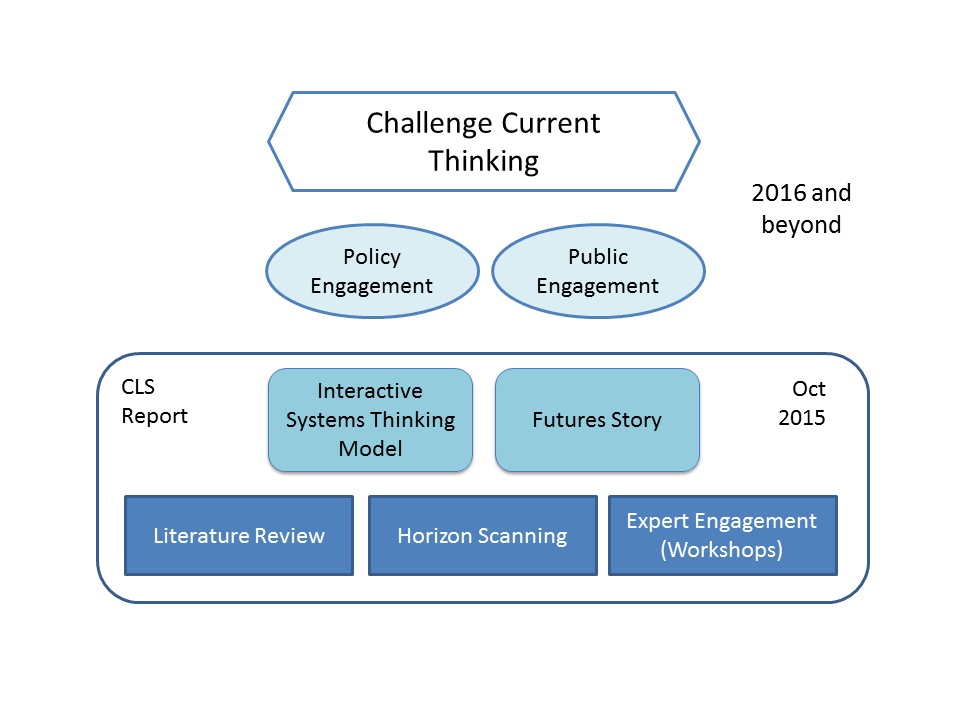
\includegraphics{img/clsSlide15.png}
\caption[Project Structure and Impact Strategy]{During 2015 the project was concluded producing the five outputs identified on this slide. In 2016 and beyond, we intend to use the tools developed in policy and public engagement on this topic and other complex public health challenges.}
\end{figure}

